\documentclass[a4paper]{report}
\usepackage{RR}
\usepackage{hyperref}
\usepackage{textcomp}
\usepackage[format=hang,width=0.8\textwidth,font={small,it},labelfont=bf]{caption}[2007/01/07]
%\usepackage[dvips]{graphicx,epsfig}
\usepackage[dvips]{epsfig}
\usepackage[dvips]{graphicx}
\usepackage{color}
\usepackage{amssymb}
\usepackage[english]{babel}
\usepackage[light,firsttwo,bottomafter]{draftcopy}
\draftcopyName{CONFIDENTIAL}{100}
%\usepackage{a4wide}
%\input{macro.tex}
\newtheorem{remark}{Remark}

\RRdate{06 Juillet 2007}
%%
\RRauthor{Pascal Denoyelle \thanks{Pascal.Denoyelle@inria.fr}
          \and
          Vincent Acary \thanks{Vincent.Acary@inria.fr}}
%%
%\authorhead{Pascal Denoyelle}
%%
\RRtitle{
		Simulation de convertisseur de puissance �lectrique � d�coupage en dynamique non-r�guli�re
		}
%% English title
\RRetitle{
        Simulation of switched mode electrical power converter with non-smooth dynamics 
	   }
%%
%\titlehead{}
%%
\RRnote{Version 1, Juillet 2007}
%%
\RRresume{
La mise au point des convertisseurs de puissance � d�coupage en �nergie �lectrique
n�cessite de simuler de plus en plus exhaustivement avant de prototyper. En effet, ces
convertisseurs sont maintenant int�gr�s avec d'autres fonctions sur un
seul circuit int�gr� dont le prototypage revient � g�n�rer les masques de fabrication
soit un co�t de l'ordre du million d'euros.

Pour concevoir des circuits bons du premier coup, l'industrie du semiconducteur
repose depuis son origine sur un ensemble d'outils logiciels parmi lesquels
les simulateurs �lectriques occupent une place importante. La r�f�rence est 
SPICE mis au point il y a 30 ans. Cependant, les convertisseurs de puissance � d�coupage
posent de gros probl�mes de convergence aux algorithmes de SPICE du fait
de commutations brutales de tension qui surviennent fr�quemment.

Nous pr�sentons ici sur un exemple les r�sultats obtenus gr�ce aux algorithmes de l'approche
non-r�guli�re qui offre un compromis vitesse de calcul~-~pr�cision remarquable.
}

\RRabstract{
The set-up of switched mode electrical power converters increasingly requires thorough
simulations before prototyping. Indeed, these converters are now being integrated with other
functions in a single integrated circuit, whose prototyping means to generate the 
photomasks i.e a cost of around one million of euros.

For designing first time good integrated circuits, semiconductor industry relies
since its beginning on a set of software tools among which electrical simulators
play a key role. The reference is SPICE that was developed 30 years ago. 
Unfortunately switched mode power converters raise severe convergence problems to SPICE algorithms
because of sudden voltage switchings frequently occurring.

We present thereafter on a test case some results that were obtained thanks to the non-smooth
approach algorithms offering a remarkable tradeoff between computation speed and
accuracy.
}
%%
\RRmotcle{convertisseur de puissance, alimentation � d�coupage, DC-DC, circuit �lectronique, nanotechnologies, simulation~num�rique,
syst�me~dynamique~non-r�gulier, LCP}

\RRkeyword{power converters, switched mode power supply, DC-DC, electronic circuit, nanotechnologies, numerical~simulation,
non-smooth~dynamical~system, LCP}

%%
\RRprojet{BIPOP}  % cas d'un seul projet
%%
\RRtheme{\THNum} % cas d'un seul theme
%%
\URRhoneAlpes % pour ceux qui sont dans les montagnes
%%

\begin{document}
\makeRT % cas d'un rapport technique.

\tableofcontents


\chapter{Introduction}
This study was focused on the simulation of a buck converter with synchronous rectification, closed-loop control 
by pulse-width modulation, loaded by a resistance or an inverter chain.
Even if this test case is a simple implementation of such converters, it involves their main functions and
it is expected that the absolute and comparative results are meaningful enough.
\\
\\
5 simulating softwares were used :
\begin{description}
\item[SICONOS :] the platform developed at INRIA Rh\^one-Alpes dealing with non-smooth dynamical systems
thanks to dedicated time integrators and algorithms to solve sets of equations and inequalities (for instance
LCP : linear complementarity problems)
\item[NGSPICE :] an open-source version of the original SPICE3F5 software developed by Berkeley university.
Even if this version may differ from existing commercial ones, it shares with them a common set of models
and the solving algorithms belong also to the same class that deals with regular functions.
\item[SMASH :] a commercial version of SPICE developed by Dolphin~Integration (see \url{http://www.dolphin.fr})
\item[ELDO :] a commercial version of SPICE with Newton-Raphson and OSR (one step relaxation) algorithms (see \cite{ELDO1985})
developed by Mentor~Graphics (\url{http://www.mentor.com}).
\item[PLECS :] a Simulink/Matlab toolbox dedicated to the simulation of power electronics circuits
(see \url{http://www.plexim.com}). The models and algorithms come from the hybrid approach.
\end{description}

SICONOS and PLECS are more oriented toward highly nonlinear circuits than SPICE versions, with a loss
of accuracy on linear or weakly nonlinear ones.
SICONOS handles dynamical systems that may involve components described by stiff, piecewise linear or even
set-valued functions. Like SPICE, it is mainly based on a time stepping integration of differential equations, but
with a specific handling of non-regular laws that may cause jumps on variables.
PLECS cuts the operation of a circuit into different modes, integrates along time within one mode while looking for 
transition events. Such events are handled separately from the time integration, whereas in SICONOS there is no
event detection.


We will now see that these differences in the approaches yield very different simulation performances.

\chapter{Test case 1 : a buck converter with a load resistor}
\section{Description of the test case modelled as a non-smooth dynamical system}
The simulated buck converter is shown in figure \ref{fig-buck-resistor}.

\begin{figure}[h]
\centerline{
  \scalebox{1.0}{
     \input{buck_resistor.pstex_t}
  }
}
\caption{Buck converter with a resistor load}
\label{fig-buck-resistor}
\end{figure}

The components are modelled with either linear or piecewise linear or set-valued relations
yielding \textbf{a non-smooth dynamical system} of the \textbf{linear time invariant
complementarity systems} class. The features of these models are given thereafter :

\begin{description}
\item[Power MOSFETS PMOS/NMOS:] they are described as an assembly of a piecewise linear current source
$I_{DS} = f(V_{GS},V_{DS})$ and the intrinsic diode ($D_{PMOS}$ and $D_{NMOS}$) with an ideal characteristic 
(see~\cite{RR-simu-elec}~chapter~4). The capacitances were not taken into account. The diodes threshold is 
$0.8~V$. The MOSFETs transconductance $KP$ was set to $10~A.V^{-2}$ and their threshold voltage to respectively
$-2~V$ for the PMOS and $2~V$ for the NMOS. One can notice that the sum of their absolute values largely exceeds 
the supply voltage $V_I~=~3~V$, thus providing non-overlapping conduction times.

\item[Compensator amplifier:] is modelled as a $10000$ gain and an output low-pass filter with a cutoff frequency of $30~MHz$.

\item[Comparator:] is modelled as a piecewise linear function whose value is $0$ if $x~<~-0.15 V$ and $V_I$
if $x~>~0.15 V$.

\item[Ramp voltage:] the frequency is $600~kHz$ and the bounds are $0$ and $0.75 \cdot ~V_I~=~2.25~V$. The rise time is
$1.655~\mu s$ and the fall time is $10~ns$.

\item[Other components:] $V_I~=~3~V$, $L~=~10~\mu H$, $C~=~22~\mu F$, load resistor $R~=~10~\Omega$, compensator :
$R_{11}~=~15.58~k \Omega$, $R_{12}~=~227.8~k \Omega$, $R_{21}~=~5.613~M \Omega$, $C_{11}~=~20~pF$, $C_{21}~=~1.9~pF$

The reference voltage $V_{ref}$ rises from $0$ to $1.8~V$ in $0.1~ms$ at the beginning of the simulation.
\end{description}
The output voltage $V_{output}$ is regulated to track the reference voltage $V_{ref}$ when $V_I$ or $V_{ref}$ or the load current
vary. The error voltage $V_{error}$ is a filtered value of the difference between $V_{output}$ and $V_{ref}$.
This voltage signal is converted into a time length thanks to a comparison with the periodic ramp signal. The comparator drives
the PMOS transistor which in turn provides more or less charge to the output depending on the error level. The operation of
a buck converter involves both a relatively slow dynamics when the switching elements (MOS and diodes) are keeping
their conducting state, and a fast dynamics when the states change. The order of magnitude are $50~ps$ for some switching details,
$1~\mu s$ for a slow variation period and $100~\mu s$ at least for a settling period of the whole circuit requiring a simulation.

\newpage
\section{Equations of the buck converter modelled as a non-smooth dynamical system}
The inductance constitutive equation is written
\[ L \cdot i_L'= -U_{DNMOS} - V_S \]

Kirchhoff Current Law (KCL) is written for several nodes, by replacing current values by the branch
constitutive equation for the linear components :
\begin{eqnarray}
i_{SDP} + i_{DNMOS} = i_L + i_{DPMOS} + i_{DSN} & \textrm{at node 2} & \label{KCLnode2}\\
i_L = C \cdot V_S' + \frac{V_S}{R} + \frac{V_S - V_{opainn}}{R_{12}}
+ \frac{V_S - V_{opainn} - U_{C_{11}} }{R_{11}} & \textrm{at node 3} & \\
\frac{V_S - V_{opainn}}{R_{12}} + \frac{V_S - V_{opainn} - U_{C_{11}} }{R_{11}}
+ \frac{U_{C_p} - U_{C_{21}} - V_{opainn}}{R_{21}} = 0 & \textrm{at node 11} & \label{KCLnode11}\\
\textrm{(input impedance of operational amplifier infinite)} & & \nonumber\\
\frac{V_S - V_{opainn} - U_{C_{11}} }{R_{11}} = C_{11} \cdot U_{C_{11}}' & \textrm{at node 12} & \\
\frac{U_{C_p} - U_{C_{21}} - V_{opainn}}{R_{21}} = C_{21} \cdot U_{C_{21}}' & \textrm{at node 13} & \\
\frac{V_{opagain} - U_{C_p}}{R_p} = C_p \cdot U_{C_p}' + \frac{U_{C_p} - U_{C_{21}} - V_{opainn}}{R_{21}} & \textrm{at node 5} & \\
\textrm{(input impedance of comparator infinite)} & & \nonumber
\end{eqnarray}
From (\ref{KCLnode11}), it comes
\[
V_{opainn} = - \frac{U_{C_{11}}}{\alpha R_{11}} - \frac{U_{C_{21}}}{\alpha R_{21}}
+ \frac{U_{C_p}}{\alpha R_{21}} + \frac{\beta V_S}{\alpha}
\]
with 
\[
\alpha = \frac{1}{R_{11}} + \frac{1}{R_{12}} + \frac{1}{R_{21}}
\]
and
\[
\beta = \frac{1}{R_{11}} + \frac{1}{R_{12}}
\]
The amplifier stage is modelled with a fixed gain $A$, thus
$V_{opagain} = A \cdot (V_{opainp} - V_{opainn})$ with $V_{opainp} = V_{ref}(t)$.
By replacing $V_{opainn}$ by its expression and grouping all differential equations, one gets :
\begin{displaymath}
\begin{array}{rrrrrrr}
V_S' = & -(\frac{1}{R C} + \frac{\beta}{\alpha R_{21} C}) V_S & + \frac{1}{C} i_L &
+ \frac{1}{C \alpha R_{21} R_{11}} U_{C_{11}} & - \frac{\beta}{\alpha R_{21} C} U_{C_{21}} &
+ \frac{\beta}{\alpha R_{21} C} U_{C_p} & \\
 & & & & & & \\
i_L'= & - \frac{1}{L} V_S & & & & & - \frac{1}{L} U_{DNMOS}\\
 & & & & & & \\
U_{C_{11}}' = & \frac{1 - \frac{\beta}{\alpha}}{\tau_{11}} V_S & & - \frac{1 - \frac{1}{\alpha R_{11}}}{\tau_{11}} U_{C_{11}} &
+ \frac{1}{\alpha R_{21} \tau_{11}} U_{C_{21}} & - \frac{1}{\alpha R_{21} \tau_{11}} U_{C_p} & \\
 & & & & & & \\
U_{C_{21}}' = & -\frac{\beta}{\alpha \tau_{21}} V_S & & + \frac{1}{\alpha R_{11} \tau_{21}} U_{C_{11}} &
- \frac{1 - \frac{1}{\alpha R_{21}}}{\tau_{21}} U_{C_{21}} & + \frac{1 - \frac{1}{\alpha R_{21}}}{\tau_{21}} U_{C_p} & \\
 & & & & & & \\
U_{C_p}' = & -\frac{A \beta}{\alpha \tau_p} V_S & & + \frac{A}{\alpha R_{11} \tau_p} U_{C_{11}} &
+ \frac{A}{\alpha R_{21} \tau_p} U_{C_{21}} & - \frac{1 + \frac{A}{\alpha R_{21}}}{\tau_p} U_{C_p} & + \frac{A}{\tau_p} V_{ref}(t)
\end{array}
\end{displaymath}
with $\tau_{11} = R_{11} C_{11}$ , $\tau_{21} = R_{21} C_{21}$ , $\tau_{p} = R_{p} C_{p}$.
\\
\\
The comparator constitutive equation is a piecewise linear model written in LCP form:
\begin{eqnarray*}
& & V_{comp} = Acomp \cdot (\lambda_{1comp} - \lambda_{2comp}) \\
& & y_{comp} = \lambda_{comp} + (U_{C_p} - V_{ramp}(t)) \cdot \left( \begin{array}{c} 1 \\ 1 \end{array} \right)
 + \left( \begin{array}{c} X1_{comp}\\X2_{comp} \end{array} \right) \\
& & 0 \leq y_{comp} \perp \lambda_{comp} \geq 0
\end{eqnarray*}
with $X1_{comp} = -0.15~V$ and $X2_{comp} = 0.15~V$ and $Acomp = \frac{V_I}{X2_{comp} - X1_{comp}}$.
\\
\\
The NMOS and PMOS constitutive equations are piecewise linear model written in LCP form:
\begin{eqnarray*}
& & i_{SDP} = \frac{K_P}{2} f_{PWLMat} \cdot (\lambda_{1PMOS} - \lambda_{2PMOS})\\
& & y_{1PMOS} = \lambda_{1PMOS} + (V_{G_{PMOS}} - V_{S_{PMOS}} - Vt_P) \cdot \left( \begin{array}{c} 1 \\ \vdots \\ 1 \end{array} \right) + vecHyp\\
& & y_{2PMOS} = \lambda_{2PMOS} + (V_{G_{PMOS}} - V_{D_{PMOS}} - Vt_P) \cdot \left( \begin{array}{c} 1 \\ \vdots \\ 1 \end{array} \right) + vecHyp\\
& & y_{PMOS} = \left( \begin{array}{c} y_{1PMOS} \\ y_{2PMOS} \end{array} \right) \\
& & \lambda_{PMOS} = \left( \begin{array}{c} \lambda_{1PMOS} \\ \lambda_{2PMOS} \end{array} \right) \\
& & 0 \leq y_{PMOS} \perp \lambda_{PMOS} \geq 0\\
\end{eqnarray*}
\\
\begin{eqnarray*}
& & i_{DSN} = \frac{K_N}{2} f_{PWLMat} \cdot (\lambda_{1NMOS} - \lambda_{2NMOS}) \\
& & y_{1NMOS} = \lambda_{1NMOS} - (V_{G_{NMOS}} - V_{S_{NMOS}} - Vt_N) \cdot \left( \begin{array}{c} 1 \\ \vdots \\ 1 \end{array} \right) + vecHyp\\
& & y_{2NMOS} = \lambda_{2NMOS} - (V_{G_{NMOS}} - V_{D_{NMOS}} - Vt_N) \cdot \left( \begin{array}{c} 1 \\ \vdots \\ 1 \end{array} \right) + vecHyp\\
& & y_{NMOS} = \left( \begin{array}{c} y_{1NMOS} \\ y_{2NMOS} \end{array} \right) \\
& & \lambda_{NMOS} = \left( \begin{array}{c} \lambda_{1NMOS} \\ \lambda_{2NMOS} \end{array} \right) \\
& & 0 \leq y_{NMOS} \perp \lambda_{NMOS} \geq 0\\
\end{eqnarray*}
The size of $y_{PMOS}$ , $\lambda_{PMOS}$ , $y_{NMOS}$ , $\lambda_{NMOS}$ is the number of breakpoints in the piecewise linear
approximation $f_{PWL}(x)$ of the function
$f(x) = \left\{ \begin{array}{ll} 0 & \textrm{if $x < 0$}\\ x^2 & \textrm{if $x \geq 0$} \end{array} \right. $.\\
Vector $vecHyp$ contains the breakpoint values sorted in ascending order.
$f_{PWLMat}$ is a one row matrix containing the values of the slope variation of $f_{PWL}(x)$ around a breakpoint.\\
\\
The intrinsic diodes $DPMOS$ and $DNMOS$ are modelled as ideal ones with thresholds $Vth_{DPMOS}$ and $Vth_{DNMOS}$ by complementarity relations.
Since $U_{DNMOS}$ appears in the inductance dynamics equation, the complementarity variable $\lambda_{DNMOS}$ is
chosen as 
\[\lambda_{DNMOS} = Vth_{DNMOS} - U_{DNMOS} \geq 0 \]
\\
Thus 
\[ y_{DNMOS} = i_{DNMOS} \geq 0 \]
and 
\[ 0 \leq y_{DNMOS} \perp \lambda_{DNMOS} \geq 0 \]

The Kirchhoff Voltage Law gives the linear relation 
\[ V_I = -U_{DPMOS} - U_{DNMOS} \]
which, by choosing
\[ y_{DPMOS} = Vth_{DPMOS} - U_{DPMOS} \geq 0 \]
is written
\[ y_{DPMOS} = -\lambda_{DNMOS} + V_I + Vth_{DPMOS} + Vth_{DNMOS} \]
\\
Thus 
\[ \lambda_{DPMOS} = i_{DPMOS} \geq 0 \]
and 
\[ 0 \leq y_{DPMOS} \perp \lambda_{DPMOS} \geq 0 \]
\\
The KCL at node 2 (\ref{KCLnode2}) gives the linear relation
\begin{eqnarray*}
y_{DNMOS} & = & i_L - i_{SDP} + i_{DSN} + i_{DPMOS}\\
y_{DNMOS} & = & i_L - \frac{K_P}{2} f_{PWLMat} \cdot (\lambda_{1PMOS} - \lambda_{2PMOS})
+ \frac{K_N}{2} f_{PWLMat} \cdot (\lambda_{1NMOS} - \lambda_{2NMOS}) + \lambda_{DPMOS}
\end{eqnarray*}
\\
By replacing in MOS transistors equations :
\begin{eqnarray*}
V_{G_{PMOS}} & = & V_{G_{NMOS}} = V_{comp} = Acomp \cdot (\lambda_{1comp} - \lambda_{2comp})\\
V_{D_{PMOS}} & = & V_{D_{NMOS}} = - U_{DNMOS} = \lambda_{DNMOS} - Vth_{DNMOS}\\
V_{S_{PMOS}} & = & V_I\\
V_{S_{NMOS}} & = & 0
\end{eqnarray*}
One gets :
\begin{eqnarray*}
& & y_{1PMOS} = \lambda_{1PMOS} + (Acomp \cdot (\lambda_{1comp} - \lambda_{2comp}) - V_I - Vt_P)
\cdot \left( \begin{array}{c} 1 \\ \vdots \\ 1 \end{array} \right) + vecHyp\\
& & y_{2PMOS} = \lambda_{2PMOS} + (Acomp \cdot (\lambda_{1comp} - \lambda_{2comp}) - \lambda_{DNMOS} + Vth_{DNMOS} - Vt_P)
\cdot \left( \begin{array}{c} 1 \\ \vdots \\ 1 \end{array} \right) + vecHyp\\
& & y_{1NMOS} = \lambda_{1NMOS} - (Acomp \cdot (\lambda_{1comp} - \lambda_{2comp}) - Vt_N)
\cdot \left( \begin{array}{c} 1 \\ \vdots \\ 1 \end{array} \right) + vecHyp\\
& & y_{2NMOS} = \lambda_{2NMOS} - (Acomp \cdot (\lambda_{1comp} - \lambda_{2comp}) - \lambda_{DNMOS} + Vth_{DNMOS} - Vt_N)
\cdot \left( \begin{array}{c} 1 \\ \vdots \\ 1 \end{array} \right) + vecHyp\\
\end{eqnarray*}
\\
All dynamical and non-smooth equations are then written in the form of an affine complementarity system~(ACS)
\begin{eqnarray*}
x' & = & A x + B \lambda + b(t) \\
y  & = & C x + D \lambda + F u(t) + e\\
0 \leq y & \perp & \lambda \geq 0
\end{eqnarray*}
with $b(t)$ and $u(t)$ source terms :
\[
b(t) = \left( \begin{array}{c} 0 \\ -\frac{Vth_{DNMOS}}{L} \\ 0 \\ 0 \\ \frac{A}{\tau_p} V_{ref}(t) \end{array} \right)
\]
and
\[
F u(t) = \left( \begin{array}{c} - V_{ramp}(t) \\ - V_{ramp}(t) \\ 0 \\ \vdots \\ 0 \end{array} \right)
\]
Matrix D belongs to class~P0 but has no symmetry property.

\section{Simulation as a non-smooth dynamical system with SICONOS}
\label{results-buck-SICO}
The start-up of the converter was simulated thanks to the SICONOS platform developed at INRIA.
As initial conditions, all state variables are zeroed.

The detailed analysis of the switching events requires to use a time step as small as~50~ps.
The simulations are carried with a fixed time step, 4000000 steps are then computed for the~$200~\mu s$~long
settling of the output voltage.

The overall result is shown on the figure \ref{fig-buck-resistor-simu-sico-0p2ms-0p05ns}.
More details of the start-up phase are shown on the figure \ref{fig-buck-resistor-simu-sico-0p01ms-0p05ns}.

The conduction times of the transistors and the NMOS intrinsic diode are visible.
\\
\\
\textbf{The CPU time required to achieve the simulation is 52~seconds on a Pentium~4 processor clocked at 3~GHz.}

\begin{figure}[hbtp]
\begin{center}
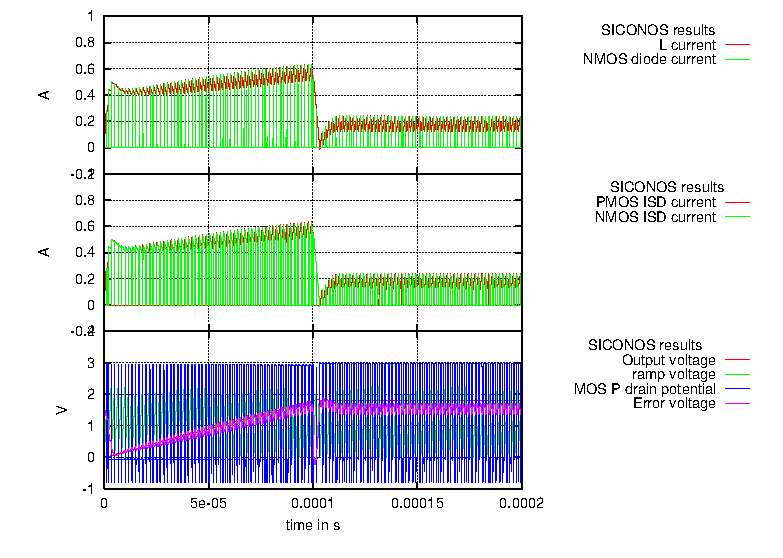
\includegraphics[scale=1.2,angle=0]{simu_siconos_0p2ms_0p05ns.eps}
\end{center}
\caption[SICONOS results, buck \protect\& load resistor (first~$200~\mu s$)]
{SICONOS simulation results, buck converter with a load resistor (first~$200~\mu s$)}
\label{fig-buck-resistor-simu-sico-0p2ms-0p05ns}
\end{figure}

\begin{figure}[hbtp]
\begin{center}
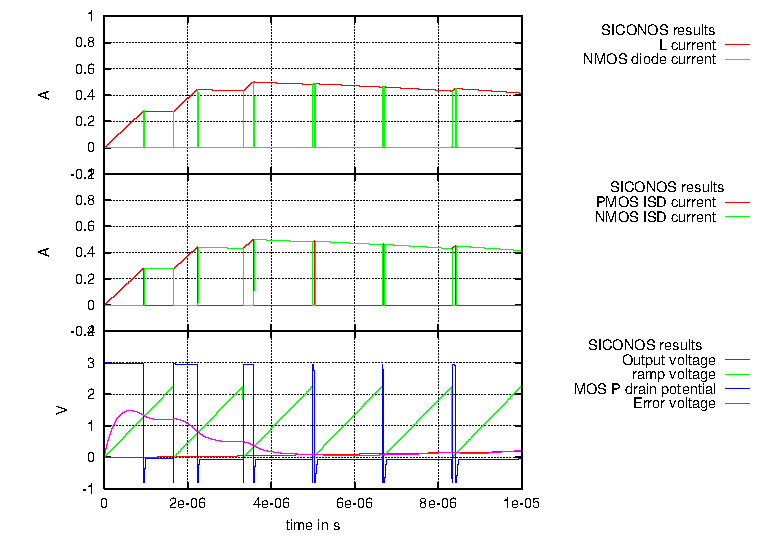
\includegraphics[scale=1.2,angle=0]{simu_siconos_0p01ms_0p05ns.eps}
\end{center}
\caption[SICONOS results, buck \protect\& load resistor (first~$10~\mu s$)]
{SICONOS simulation results, buck converter with a load resistor (first~$10~\mu s$)}
\label{fig-buck-resistor-simu-sico-0p01ms-0p05ns}
\end{figure}

Some configuration parameters (namely a small LC value and a high value of the high
frequency compensator gain) may yield multiple crossings of the error voltage with the
ramp voltage within one period. The robustness of the non-smooth modelling and solving algorithms enables to perform
with the same CPU time the simulation of such cases. For instance, figures \ref{fig-buck-resistor-simu-sico-std}, 
\ref{fig-buck-resistor-simu-sico-lowLC} and \ref{fig-buck-resistor-simu-sico-lowLC-badcomp} 
show the effect of reducing $L$ to $4~\mu H$, $C$
to $10~\mu F$ (yielding double crossings along one ramp period) and then to change $R_{11}$ to $10~K\Omega$, $R_{21}$ to $8~M\Omega$, $C_{11}$ to $10~pF$ (yielding a sliding mode).

\begin{figure}[hbtp]
\begin{center}
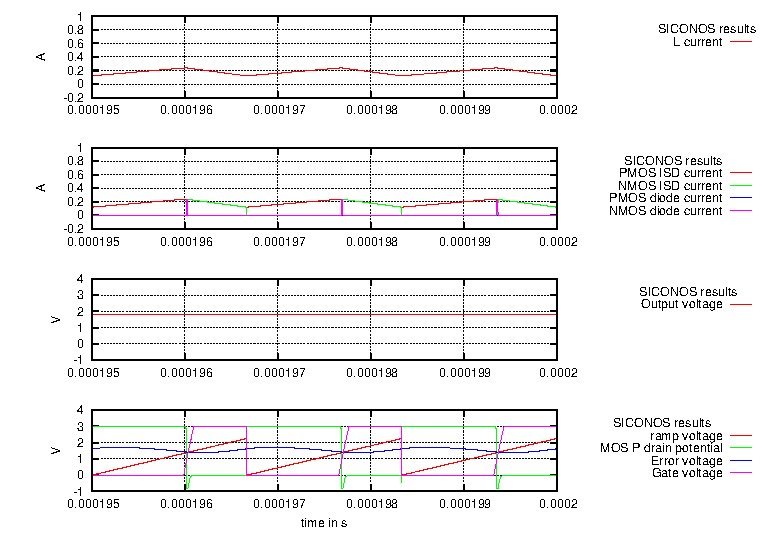
\includegraphics[scale=1.2,angle=0]{simu_siconos_standard.eps}
\end{center}
\caption[SICONOS results, buck \protect\& load resistor , steady state , simple crossings]
{SICONOS simulation results, buck converter with a load resistor\protect\newline
steady state with standard parameters}
\label{fig-buck-resistor-simu-sico-std}
\end{figure}

\begin{figure}[hbtp]
\begin{center}
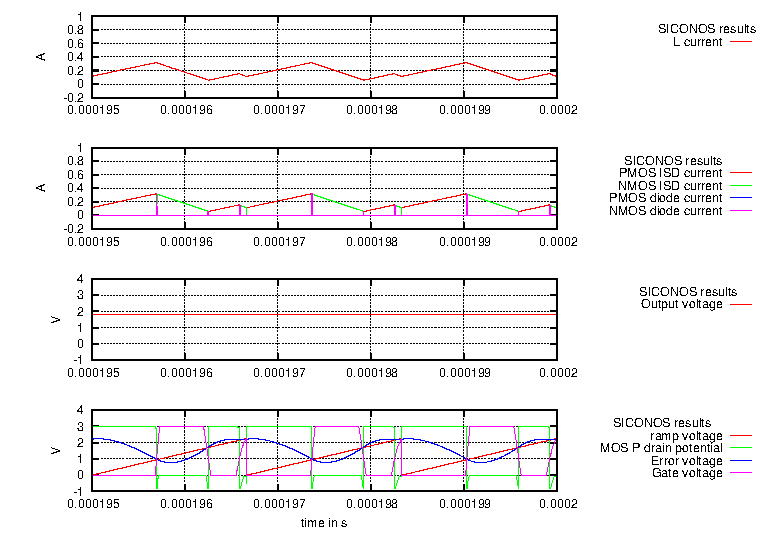
\includegraphics[scale=1.2,angle=0]{simu_siconos_lowLC.eps}
\end{center}
\caption[SICONOS results, buck \protect\& load resistor , steady state , double crossings]
{SICONOS simulation results, buck converter with a load resistor\protect\newline
steady state with $L~=~4~\mu H$, $C~=~10~\mu F$}
\label{fig-buck-resistor-simu-sico-lowLC}
\end{figure}

\begin{figure}[hbtp]
\begin{center}
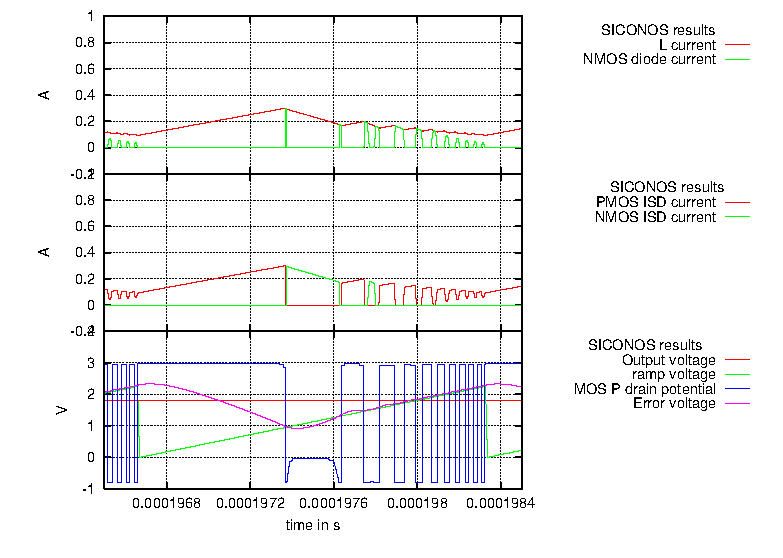
\includegraphics[scale=1.2,angle=0]{simu_siconos_lowLC_badcomp.eps}
\end{center}
\caption[SICONOS results, buck \protect\& load resistor , steady state , sliding mode]
{SICONOS simulation results, buck converter with a load resistor\protect\newline
steady state with $L~=~4~\mu H$, $C~=~10~\mu F$ , $R_{11}~=~10~K\Omega$, $R_{21}~=~8~M\Omega$, $C_{11}~=~10~pF$\protect\newline
exhibiting a sliding mode}
\label{fig-buck-resistor-simu-sico-lowLC-badcomp}
\end{figure}

\clearpage

\section{Simulation with SPICE : convergence issues related to the MOS model}
\subsection{Simulation conditions}
The simulation of this circuit was done with several versions of SPICE (the open source NGSPICE from Berkeley, SMASH from Dolphin and
ELDO from Mentor Graphics) and two kinds of MOS models :
\begin{description}
\item[the MOS level 3 model :] this model was preferred to the MOS level 1 since it allowed the convergence
of the SMASH simulator with the requirement to add a small capacitor between ground and node 2 (connection between
the MOS transistors). This model takes more physical effects into account than the piecewise linear model used in SICONOS simulations,
in particular the voltage-dependent capacitances. It is an important issue since these varying capacitances
cause some convergence problems when node 2 switches between $V_I$ and ground.
Adding a small capacitor of a few picoFarad between this node and ground helps to solve the problem
but may yield artifacts (spikes) on the current of the~$V_I$~alim and the MOS transistors.
\item[a simplified model (Sah model)] with fixed capacitances and a quadratic static characteristic :
\[
I_{DS} = \textrm{max}(0,V_{GS}-Vt_N)^2 - \textrm{max}(0,V_{GD}-Vt_N)^2 \qquad \textrm{for an NMOS}
\]
This model is very close to the piecewise linear model used in SICONOS simulations. The implementation in netlists was done thanks to 
voltage-dependent current sources that are very likely not compiled by the various SPICE simulators tested.
Thus the CPU time measured is increased with respect to a compiled version of the same model.
An estimation of the CPU time with a compiled simplified model is given by multiplying the MOS level 3 CPU time
by the ratio of the Newton-Raphson iterations required respectively during the simulations with each model.
An additional correction should be done to reflect that the computation of the jacobian matrix entries
linked to a compiled simplified model would require less time than with a MOS level 3 model. Even if the SPICE simulation
includes other operations, jacobian matrix loading time is indeed known to be generally predominant.
\end{description}


\begin{itemize}
\item Power MOSFETS intrinsic diodes are modelled by the classical Shockley equation with an emission
coefficient $N~=~1$ :
\[ I = I_S.({e^{\frac{q.V}{N.k.T}} - 1}) \qquad \textrm{when} \quad V > -5.N.\frac{k.T}{q} \]
\[ I = -I_S \qquad  \textrm{when} \quad V < -5.N.\frac{k.T}{q} \]
with
\[
\begin{array}{ll}
V\,,\,I & \textrm{voltage across the diode and current through the diode}\\
I_S & \textrm{saturation current, default value $10^{-14}$~A}\\
q & \textrm{electron charge $1.6\,10^{-19}$~C}\\
k & \textrm{Boltzmann constant $1.38\,10^{-23}\,J.K^{-1}$}\\
T & \textrm{temperature in K}\\
N & \textrm{emission coefficient}
\end{array}
\]
\item The comparator is modelled as a non linear voltage controlled voltage source defined as $V_{out}~=~1.5~\cdot~(tanh(10~\cdot~V_{in}) + 1)$.
Thus the 3~segment characteristic used as the non smooth model is regularized to help convergence of SPICE
(see a comparison of the PWL comparator as used in SICONOS simulations with the SPICE one in figure \ref{fig-comparator-models}).
\end{itemize}

\begin{figure}[hbtp]
\begin{center}
\includegraphics[scale=1.0,angle=0]{comparators.eps}
\end{center}
\caption{Comparison of PWL and SPICE (tanh based) comparator models}
\label{fig-comparator-models}
\end{figure}

\clearpage

The power supply $V_I$ is raised from 0 in $50~ns$ at the beginning to help the convergence.\footnote{This is
not required with the SICONOS algorithms that find a consistent initial solution from scratch.}
The SPICE tolerance values used are $1~nA$ for currents, $1~\mu V$ for voltages and $0.00075$ for relative differences.
The maximum number of Newton-Raphson iterations is set to 100 (the default values are 10 for NGSPICE, 20 for SMASH and
13 for ELDO).

Usually, SPICE simulators integrate time with a time step adjusted according to different strategies based on an estimation
of the local truncation error (LTE) or the number of Newton-Raphson iterations required by previous steps.
Since SICONOS simulations were carried with a fixed time step of~50~ps, simulators were forced to use this value as a maximum.
Even when SPICE simulators use fixed time step, they may compute LTE to assess a solution found by the Newton-Raphson
algorithm. This computation of LTE was disabled because it could impair the performance of SPICE with respect to SICONOS.
\footnote{For NGSPICE, it implied a slight modification of the source code since no standard option is provided to do it.}

\subsection{Simulation results}
The following tables displays the results with the standard and the sliding mode values of compensator components
(see \ref{results-buck-SICO}). An estimation of the CPU time with a compiled simplified model is added.
\\
\\
\begin{tabular}{|l|c|r|r|r|r|}
\hline
\multicolumn{6}{|c|}{\textbf{standard compensator values}}\\
\hline
simulator & model & time steps & NR iterations & CPU time (s) & CPU time estimation (s)\\
\hline
NGSPICE & simple  & 4000000 & 8024814 & 632 & 357\\
NGSPICE & level 3 & 4000000 & 8304237 & 370 & \\
\hline
SMASH   & simple  & 4000404 & 8073070 & 230 & 172\\
SMASH   & level 3 & 4000323 & 8059868 & 172 & \\
\hline
ELDO    & simple  & 4000000 & 4547579 & 388 & 355\\
ELDO    & level 3 & 4000000 & 4554452 & 356 & \\
\hline
\end{tabular}
\begin{tabular}{|l|c|r|r|r|r|}
\hline
\multicolumn{6}{|c|}{\textbf{sliding mode compensator values}}\\
\hline
simulator & model & time steps & NR iterations & CPU time (s) & CPU time estimation (s)\\
\hline
NGSPICE & simple  & 4000000 & 8070324 & 638 & 358\\
NGSPICE & level 3 & 4000000 & 8669053 & 385 & \\
\hline
SMASH   & simple  & 4000252 & 8239697 & 234 & 176\\
SMASH   & level 3 & 4000131 & 8220181 & 176 & \\
\hline
ELDO    & simple  & 4000000 & 5861226 & 438 & 365\\
ELDO    & level 3 & 4000000 & 5888994 & 367 & \\
\hline
\end{tabular}
\\
\\
These results shall be compared to the 52~s~CPU time achieved with the non-smooth dynamics.
Depending on the model and the SPICE simulator, the (estimated) CPU time is from~3.3~to~7.4
larger than with SICONOS.\\

Moreover, it was necessary to add a parasitic capacitor on the connection between the PMOS and NMOS
transistors to allow the convergence of the SMASH simulator with both models of MOS
and of the NGSPICE simulator with the MOS level 3 model.

The overall result obtained with NGSPICE and the simplified model is shown on the figure \ref{fig-buck-resistor-simu-ngspice-0p2ms-0p05ns}.
More details of the start-up phase are shown on the figure \ref{fig-buck-resistor-simu-ngspice-0p01ms-0p05ns}.

\begin{figure}[hbtp]
\begin{center}
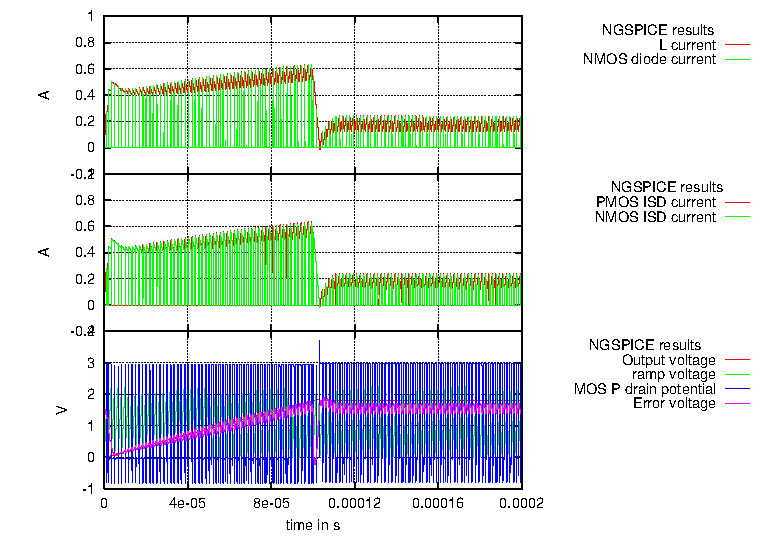
\includegraphics[scale=1.2,angle=0]{simu_ngspice_0p2ms_0p05ns.eps}
\end{center}
\caption[NGSPICE results, buck \protect\& load resistor (first~$200~\mu s$)]
{NGSPICE simulation results, buck converter with a load resistor (first~$200~\mu s$)}
\label{fig-buck-resistor-simu-ngspice-0p2ms-0p05ns}
\end{figure}

\begin{figure}[hbtp]
\begin{center}
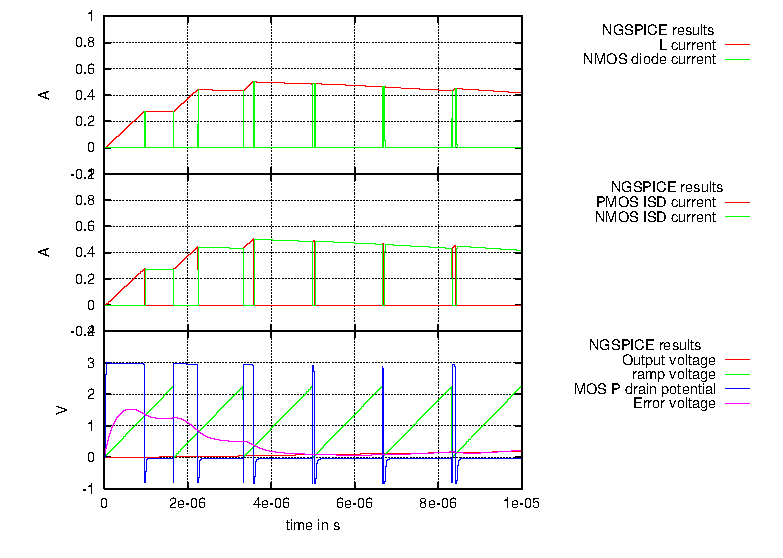
\includegraphics[scale=1.2,angle=0]{simu_ngspice_0p01ms_0p05ns.eps}
\end{center}
\caption[NGSPICE results, buck \protect\& load resistor (first~$10~\mu s$)]
{NGSPICE simulation results, buck converter with a load resistor (first~$10~\mu s$)}
\label{fig-buck-resistor-simu-ngspice-0p01ms-0p05ns}
\end{figure}

\clearpage
The detailed analysis of a ramp cycle with standard component values and sliding mode related values as shown on
\ref{fig-buck-resistor-simu-sico-std} and \ref{fig-buck-resistor-simu-sico-lowLC-badcomp} are displayed on
figures \ref{fig-buck-resistor-simu-ngspice-std} and \ref{fig-buck-resistor-simu-ngspice-lowLC-badcomp}.\\

The overall functioning during one ramp in the standard case is now described
(see~\ref{fig-buck-resistor-simu-sico-std} and~\ref{fig-buck-resistor-simu-ngspice-std}):\\
At the end of the previous ramp period (time~$196.6~\mu s$),
the fast falling ramp signal crosses the error signal which results in the end of the NMOS conduction period
and the beginning of the PMOS one. During the very short time (around~250~ps) when no MOS conducts, the NMOS intrinsic
diode allows the current to flow through the inductance : this yields the spike on the NMOS diode current visible
on the top chart of~\ref{fig-buck-resistor-simu-sico-std}~and~\ref{fig-buck-resistor-simu-ngspice-std}.
In the middle of the ramp period (time~$197.7~\mu s$),
the slowly rising ramp signal crosses the error signal which results in the end of the PMOS conduction period
and the beginning of the NMOS one. There is also an intermediate period when no MOS conducts and the NMOS intrinsic
diode acts as freewheeling (or flyback). It lasts longer due to the slower variation of voltages. These diode
conducting periodes are also visible on the bottom chart on the PMOS drain potential : during NMOS diode conduction,
this potential is clamped to~$-0.8~V$ according to the diode threshold voltage.\\

One can notice that SICONOS and NGSPICE simplified model results are very close.

\begin{figure}[hbtp]
\begin{center}
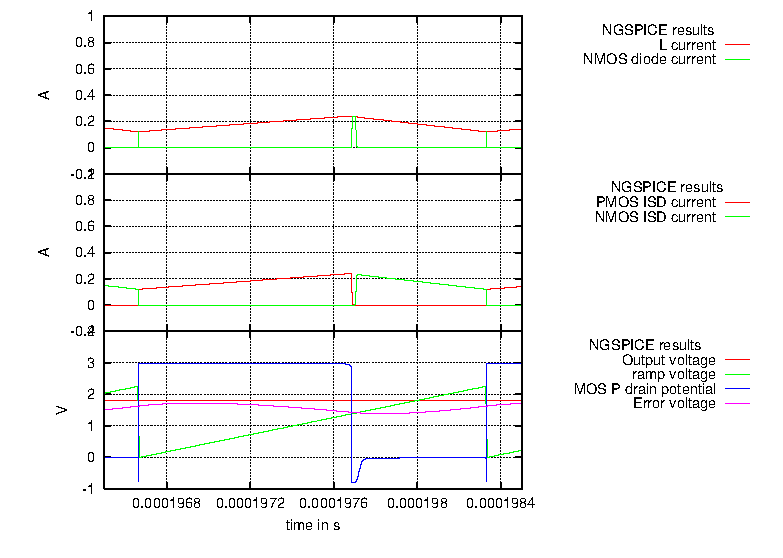
\includegraphics[scale=1.2,angle=0]{simu_ngspice_standard.eps}
\end{center}
\caption[NGSPICE results, buck \protect\& load resistor , steady state , simple crossings]
{NGSPICE simulation results, buck converter with a load resistor\protect\newline
steady state with standard parameters}
\label{fig-buck-resistor-simu-ngspice-std}
\end{figure}

\begin{figure}[hbtp]
\begin{center}
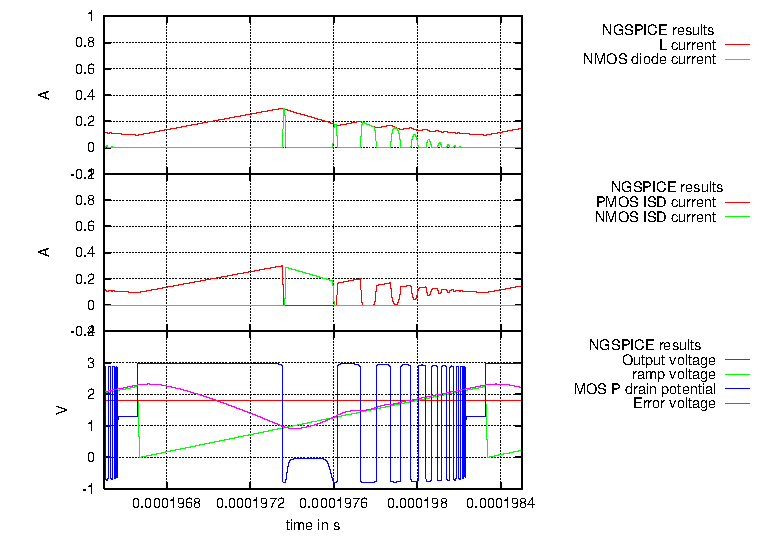
\includegraphics[scale=1.2,angle=0]{simu_ngspice_lowLC_badcomp.eps}
\end{center}
\caption[NGSPICE results, buck \protect\& load resistor , steady state , sliding mode]
{NGSPICE simulation results, buck converter with a load resistor\protect\newline
steady state with $L~=~4~\mu H$, $C~=~10~\mu F$ , $R_{11}~=~10~K\Omega$, $R_{21}~=~8~M\Omega$, $C_{11}~=~10~pF$\protect\newline
exhibiting a sliding mode}
\label{fig-buck-resistor-simu-ngspice-lowLC-badcomp}
\end{figure}

\clearpage
Figure \ref{fig-compar-Sah-level3} shows the results over one ramp period with the simplified versus level 3 MOS models,
where both simulations were performed with ELDO (the only SPICE simulator converging with the level 3 model
without extra capacitor). There is no noticeable difference.

\begin{figure}[hbtp]
\begin{center}
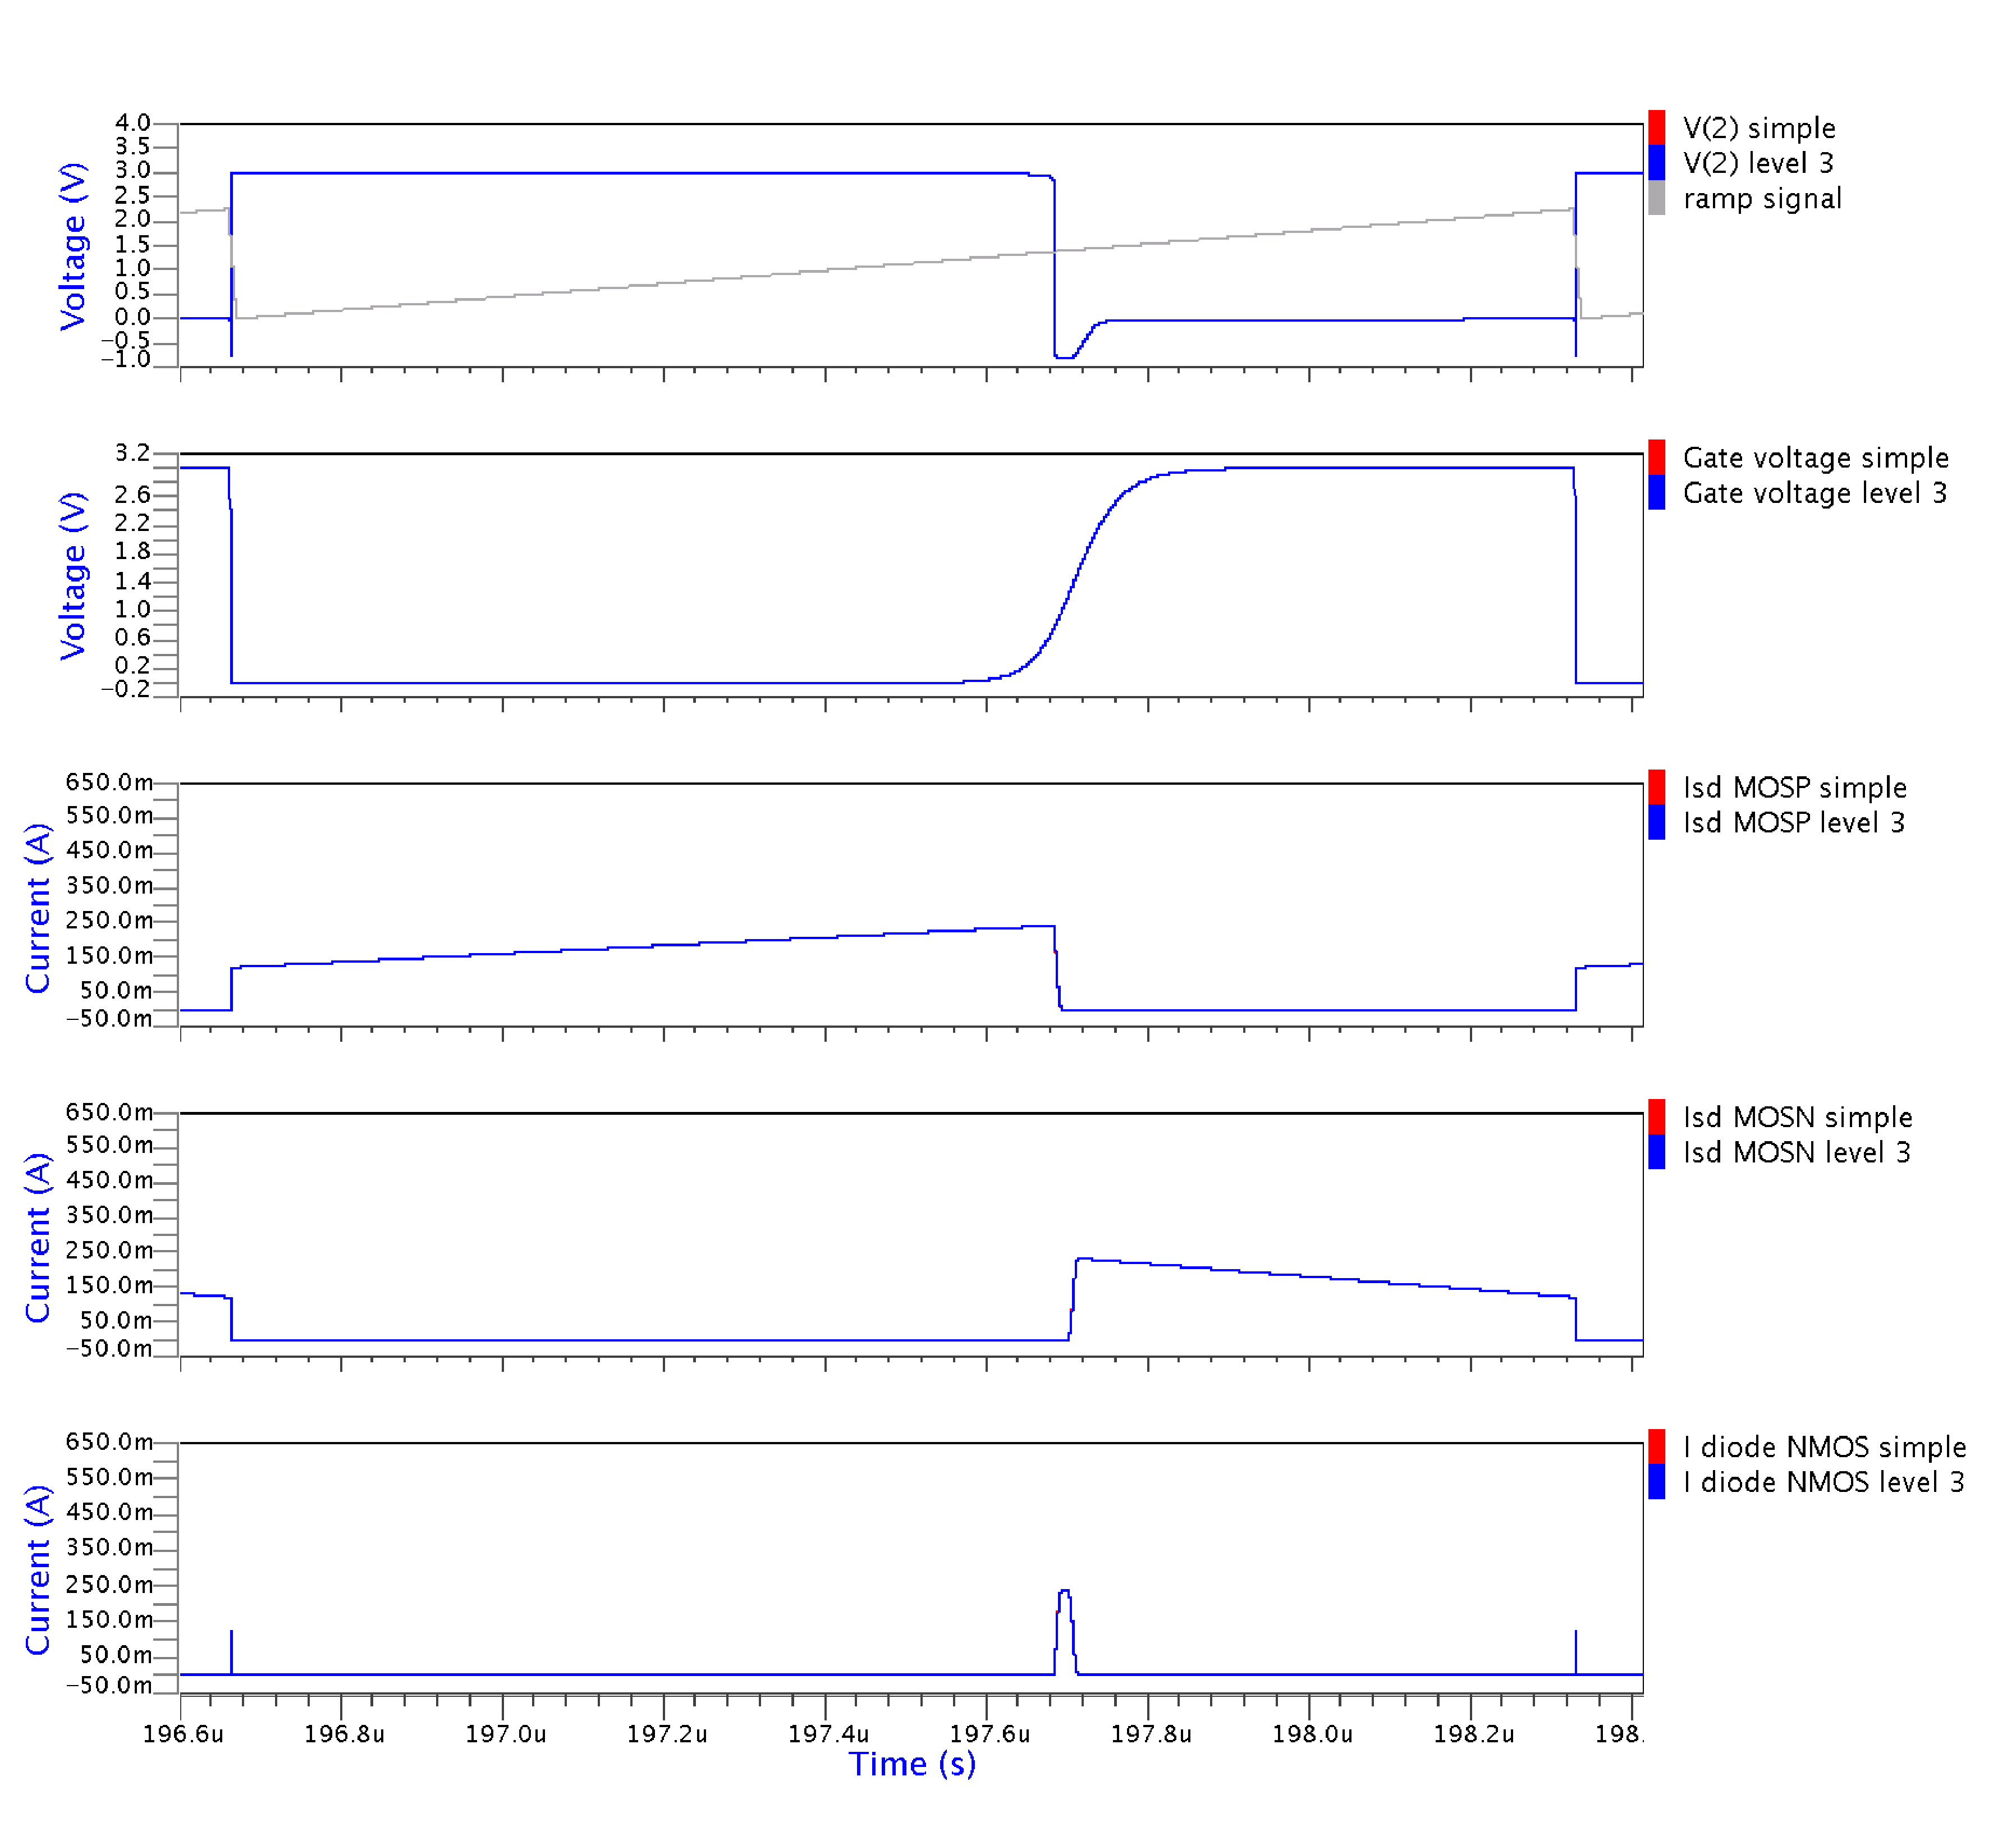
\includegraphics[scale=0.25,angle=0]{compar_Sah_level3.eps}
\end{center}
\caption
{Simplified vs. level 3 MOS models ELDO results (one ramp in steady state)}
\label{fig-compar-Sah-level3}
\end{figure}

\clearpage

\section{Simulation with PLECS}

PLECS is a Simulink/Matlab toolbox dedicated to the simulation of power electronics circuits.
(see \url{http://www.plexim.com}). The electronic circuits are modelled as hybrid systems:
at each instant, the circuit is described according to one of a set of topologies specified
by the ON or OFF state of ideal switches (diodes, transistors\dots). A topology is
valid when the computed value of some variables (for instance a diode current or voltage) is kept within some
bounds. When a topology is no more valid, a new topology has to be found as well as the possible jump
of variables linked to this topology switching. Even if this approach targets the same kind of systems
as the non-smooth dynamics, its models and algorithms differ mainly in :\\
\\
\begin{tabular}{|p{6cm}|p{6cm}|}
\hline
\textbf{Hybrid systems} & \textbf{Non-smooth dynamical systems} \\
\hline
Each topology is described by a separate set of equations. & 
A single set of equations and constraints describes the whole system. \\
 & \\
Checking the topology switching conditions is critical and may be computationally expensive. &
There is no topology switching : constraints are met at each time step. \\
 & \\
Determining the new topology and the new state value after a topology switch is not obvious.
It may be quick if it can benefit from prior knowledge about the circuit's operation but may also involve heavy computations to check
all possible transitions if no rule is available. &
At each time step, the new values are computed to meet equations and constraints thanks to proper
time integration schemes and one step problem solving based on optimization algorithms \\
\hline
\end{tabular}
\\
\\
The switch models (diodes and transistors) available in the PLECS toolbox are ideal : the transistors
are supposed to be controlled by a boolean signal forcing a conducting or blocking state. 
The power NMOS and PMOS are controlled by opposite signals issued from the feedback loop, thus there is no
flyback conduction by the NMOS intrinsic diode (see description of the PLECS circuit and the Simulink model in appendix
\ref{modele-PLECS-buckresistor}).
\\
\\
\textbf{The CPU time required to achieve the simulation of $200~\mu s$ ranges between $135~s$ and $410~s$ on a 
Pentium~4 clocked at 3~GHz, depending on the values of the resistors, capacitors and inductor.} This should be compared
to the $52~s$ of the SICONOS simulation, \textbf{obtained independently from these components values}. This demonstrates
the robustness and efficiency of the time-stepping scheme and the one step solving algorithms of SICONOS. Moreover, the
short time step (50~ps) used in SICONOS simulations was required to catch some conduction periods of the NMOS intrinsic
diode. As explained above, these phenomena are not simulated with the present PLECS circuit.

Figures \ref{fig-buck-resistor-simu-plecs-0p2ms-std} and \ref{fig-buck-resistor-simu-plecs-zoom-std} show the results
when the standard parameters are used : $L~=~10~\mu H$, $C~=~22~\mu F$, $R_{11}~=~15.58~k \Omega$, $R_{12}~=~227.8~k \Omega$,
$R_{21}~=~5.613~M \Omega$, $C_{11}~=~20~pF$, $C_{21}~=~1.9~pF$.

Figures \ref{fig-buck-resistor-simu-plecs-0p2ms-sliding} and \ref{fig-buck-resistor-simu-plecs-zoom-sliding} show the results
when the parameters yielding a sliding mode are used : $L~=~4~\mu H$, $C~=~10~\mu F$, $R_{11}~=~10~k \Omega$, $R_{12}~=~227.8~k \Omega$,
$R_{21}~=~8~M \Omega$, $C_{11}~=~10~pF$, $C_{21}~=~1.9~pF$.

\begin{figure}[hbtp]
\begin{center}
\includegraphics[scale=0.8,angle=270]{simu_plecs_buckresistor_std0p2ms.eps}
\end{center}
\caption[PLECS results, buck \protect\& load resistor , simple crossings]
{PLECS simulation results, buck converter with a load resistor\protect\newline
standard parameters}
\label{fig-buck-resistor-simu-plecs-0p2ms-std}
\end{figure}

\begin{figure}[hbtp]
\begin{center}
\includegraphics[scale=0.8,angle=270]{simu_plecs_buckresistor_stdzoom.eps}
\end{center}
\caption[PLECS results, buck \protect\& load resistor , steady state , simple crossings]
{PLECS simulation results, buck converter with a load resistor\protect\newline
standard parameters (zoom view of steady state)}
\label{fig-buck-resistor-simu-plecs-zoom-std}
\end{figure}

\begin{figure}[hbtp]
\begin{center}
\includegraphics[scale=0.8,angle=270]{simu_plecs_buckresistor_sliding0p2ms.eps}
\end{center}
\caption[PLECS results, buck \protect\& load resistor , sliding mode]
{PLECS simulation results, buck converter with a load resistor\protect\newline
$L~=~4~\mu H$, $C~=~10~\mu F$ , $R_{11}~=~10~K\Omega$, $R_{21}~=~8~M\Omega$, $C_{11}~=~10~pF$\protect\newline
exhibiting a sliding mode}
\label{fig-buck-resistor-simu-plecs-0p2ms-sliding}
\end{figure}

\begin{figure}[hbtp]
\begin{center}
\includegraphics[scale=0.8,angle=270]{simu_plecs_buckresistor_slidingzoom.eps}
\end{center}
\caption[PLECS results, buck \protect\& load resistor , steady state , sliding mode]
{PLECS simulation results, buck converter with a load resistor\protect\newline
$L~=~4~\mu H$, $C~=~10~\mu F$ , $R_{11}~=~10~K\Omega$, $R_{21}~=~8~M\Omega$, $C_{11}~=~10~pF$\protect\newline
exhibiting a sliding mode (zoom view of ``steady'' state)}
\label{fig-buck-resistor-simu-plecs-zoom-sliding}
\end{figure}

\clearpage
\chapter{Test case 2 : a buck converter loaded by a resistor and an inverter chain}
An inverter chain is supplied by the converter in parallel with the resistor. The input of 
this chain starts to oscillate between $0$ and $1.8~V$ after $150~\mu s$, i.e~$50~\mu s$
after the reference voltage reaches $1.8~V$.

The simulated circuit is shown in figure \ref{fig-buck-inverters}.

\begin{figure}[h]
\centerline{
  \scalebox{0.8}{
     \input{buck_inverters.pstex_t}
  }
}
\caption{Buck converter supplying a resistor load and an inverter chain}
\label{fig-buck-inverters}
\end{figure}

\section{Simulation as a non-smooth dynamical system with SICONOS}
\label{section-simu-siconos-buckinv}
The inverter MOSFETs are modelled with a piecewise linear characteristic~$I_{DS}~=~f(V_{GS},V_{DS})$.
Their parameters are:
\begin{description}
\item[Transconductance $KP$:] $4.3\cdot10^{-5}~A.V^{-2}$ for the PMOS , $12.9\cdot10^{-5}~A.V^{-2}$ for the NMOS
\item[Threshold voltage:] $-0.6~V$ for the PMOS and $0.6~V$ for the NMOS
\item[Output capacitive load :] $20~fF$
\end{description}

Two chain lengths were tested :

In the first case, the chain includes only 2 inverters to enable a CPU time comparison with PLECS
whose evaluation version is limited to 6~switches.
To emulate a large current drawn from the output of the converter, the 2 inverters chain
is supposed to be~8000~times large, i.e~8000~chains switching simultaneously as a synchronous
logic circuit. The transconductance and capacitance are therefore multiplied by~8000. The
switching frequency of the chain input is~$200~MHz$.
\\
\\
\textbf{The CPU time required to achieve the simulation of~$200~\mu s$ with a~50~ps time step
is 110~seconds on a Pentium~4 clocked at 3~GHz.}
\\
Results are displayed in figures \ref{fig-buck-inverter-simu-sico-0p2ms-0p05ns} and 
\ref{fig-buck-inverter-simu-sico-zoom1}. Figure \ref{fig-buck-inverter-simu-sico-zoom1}
shows the start-up of the inverters switching.
\\
\begin{figure}[hbtp]
\begin{center}
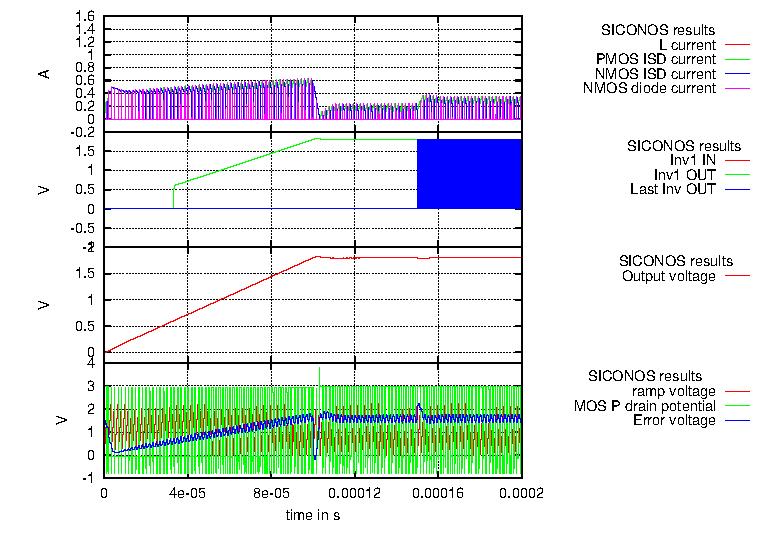
\includegraphics[scale=1.2,angle=0]{simu_siconos_buck2inv_0p2ms_0p05ns.eps}
\end{center}
\caption[SICONOS results, buck \protect\& load resistor \protect\& inverters (first~$200~\mu s$)]
{SICONOS simulation results, buck converter supplying a load resistor and an inverter chain (first~$200~\mu s$)}
\label{fig-buck-inverter-simu-sico-0p2ms-0p05ns}
\end{figure}

\begin{figure}[hbtp]
\begin{center}
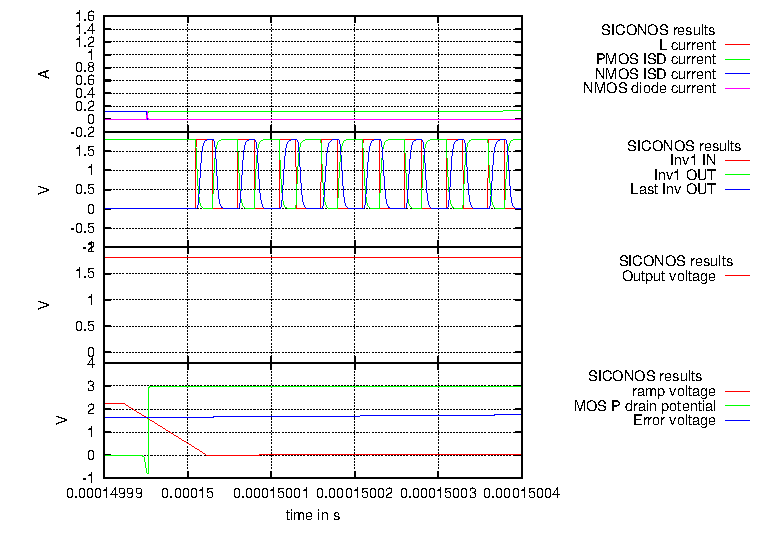
\includegraphics[scale=1.2,angle=0]{simu_siconos_buck2inv_zoom1.eps}
\end{center}
\caption[SICONOS results, buck \protect\& load resistor \protect\& inverters (zoom)]
{SICONOS simulation results, buck converter supplying a load resistor and an inverter chain\protect\newline
Zoom on the start-up of the inverter chain}
\label{fig-buck-inverter-simu-sico-zoom1}
\end{figure}

\clearpage

A 50 inverters long chain was also simulated with transconductance and capacitance multiplied by~320.
\\
\textbf{The CPU time required to achieve the simulation of~$200~\mu s$ with a~50~ps time step
is~2~hours~31~minutes on a Pentium~4 clocked at 3~GHz.}
\\
The large increase in CPU time is due to
the lack of sparse matrix techniques in the current implementation of SICONOS. Sparse matrices
are widely used in SPICE simulators since electronic circuits yield frequently sparsity
factors (i.e~ratio of zero terms) of~0.9. For instance, at least 92~\% of the jacobian matrix terms
are zero in the considered circuit of a buck converter with 50~inverters. The LCP~matrix used in
SICONOS simulation is also sparse by 92~\%. Obviously, using sparse matrices will greatly reduce
the SICONOS CPU time since many matrix-vector products are computed.

Figure \ref{fig-buck-50inverter-simu-sico-compdelays} shows a detail of this simulation : it compares
the switching instants of the chain output $2~\mu s$ after the clock starts and $16~\mu s$ later. $2~\mu s$ after
the clock starts, the buck converter output voltage that supplies the inverter chain drops by~10~mV due to the
sudden increase of power consumption. $16~\mu s$ later, the output voltage is again equal to the prescribed
value~1.8~V thanks to the regulation. This tiny variation has an impact on the inverters delays, a smaller supply
voltage yielding an increase of delay. This behaviour is well analyzed in the SICONOS simulation thanks to the
modelling of the voltage-dependent current through the MOS transistors.

\begin{figure}[hbtp]
\begin{center}
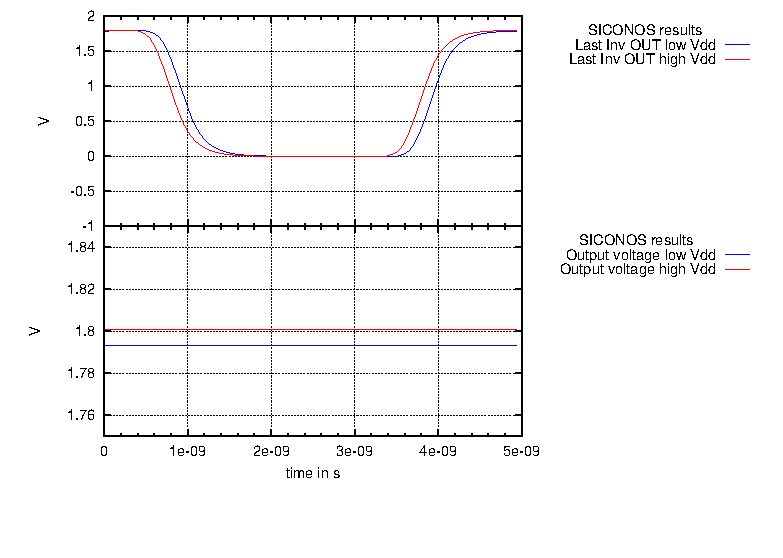
\includegraphics[scale=1.2,angle=0]{simu_siconos_buck50inv_invdelays.eps}
\end{center}
\caption[SICONOS results, buck \protect\& load resistor \protect\& 50 inverters (zoom)]
{SICONOS simulation results, buck converter supplying a load resistor and a 50 inverters chain\protect\newline
Chain delay variation linked to the converter output voltage}
\label{fig-buck-50inverter-simu-sico-compdelays}
\end{figure}

\clearpage

\section{Simulation with SPICE (ELDO)}
The circuit was simulated with ELDO, the only available SPICE simulator that converges with
the buck netlist instantiating as power MOS a classical (level 3) MOS model without requiring to add
parasitic capacitances. Simulations were done with a~50~ps~time step and no~LTE estimation.
\\
\\
\textbf{The simulation of the buck with a 2 inverters chain takes 439~s on a Pentium~4 clocked at 3~GHz.}
\\
\textbf{The simulation of the buck with a 50 inverters chain takes 25~minutes on a Pentium~4 clocked at 3~GHz.}
\\
With 2 inverters only, SICONOS runs 4~times faster whereas with~50~inverters, ELDO runs 6~times faster.
These are initial results since :
\begin{itemize}
\item as explained in \ref{section-simu-siconos-buckinv}, the SICONOS run time
will benefit from the use of sparse matrix techniques.
\item the present representation of the circuit as a non-smooth dynamical system replaces every
non-linear component by set-valued or piecewise linear functions yielding an LCP. It is possible to mix such
models with classical smooth models like SPICE ones, resulting in a NLCP. The detailed analysis of an
inverter chain is better handled if MOS transistors are modelled with classical smooth functions because
a precise piecewise linear model yields a too large LCP. Best results could be reached by mixing smooth
and non-smooth models. This is possible since both formulations are based on differential equations
and thanks to NLCP solvers.
\end{itemize}

Results are displayed in figures \ref{fig-buck-inverter-simu-ELDO-0p2ms-0p05ns} and
\ref{fig-buck-inverter-simu-ELDO-zoom1}. Figure \ref{fig-buck-inverter-simu-ELDO-zoom1}
shows the start-up of the inverters switching.
\\
\begin{figure}[hbtp]
\begin{center}
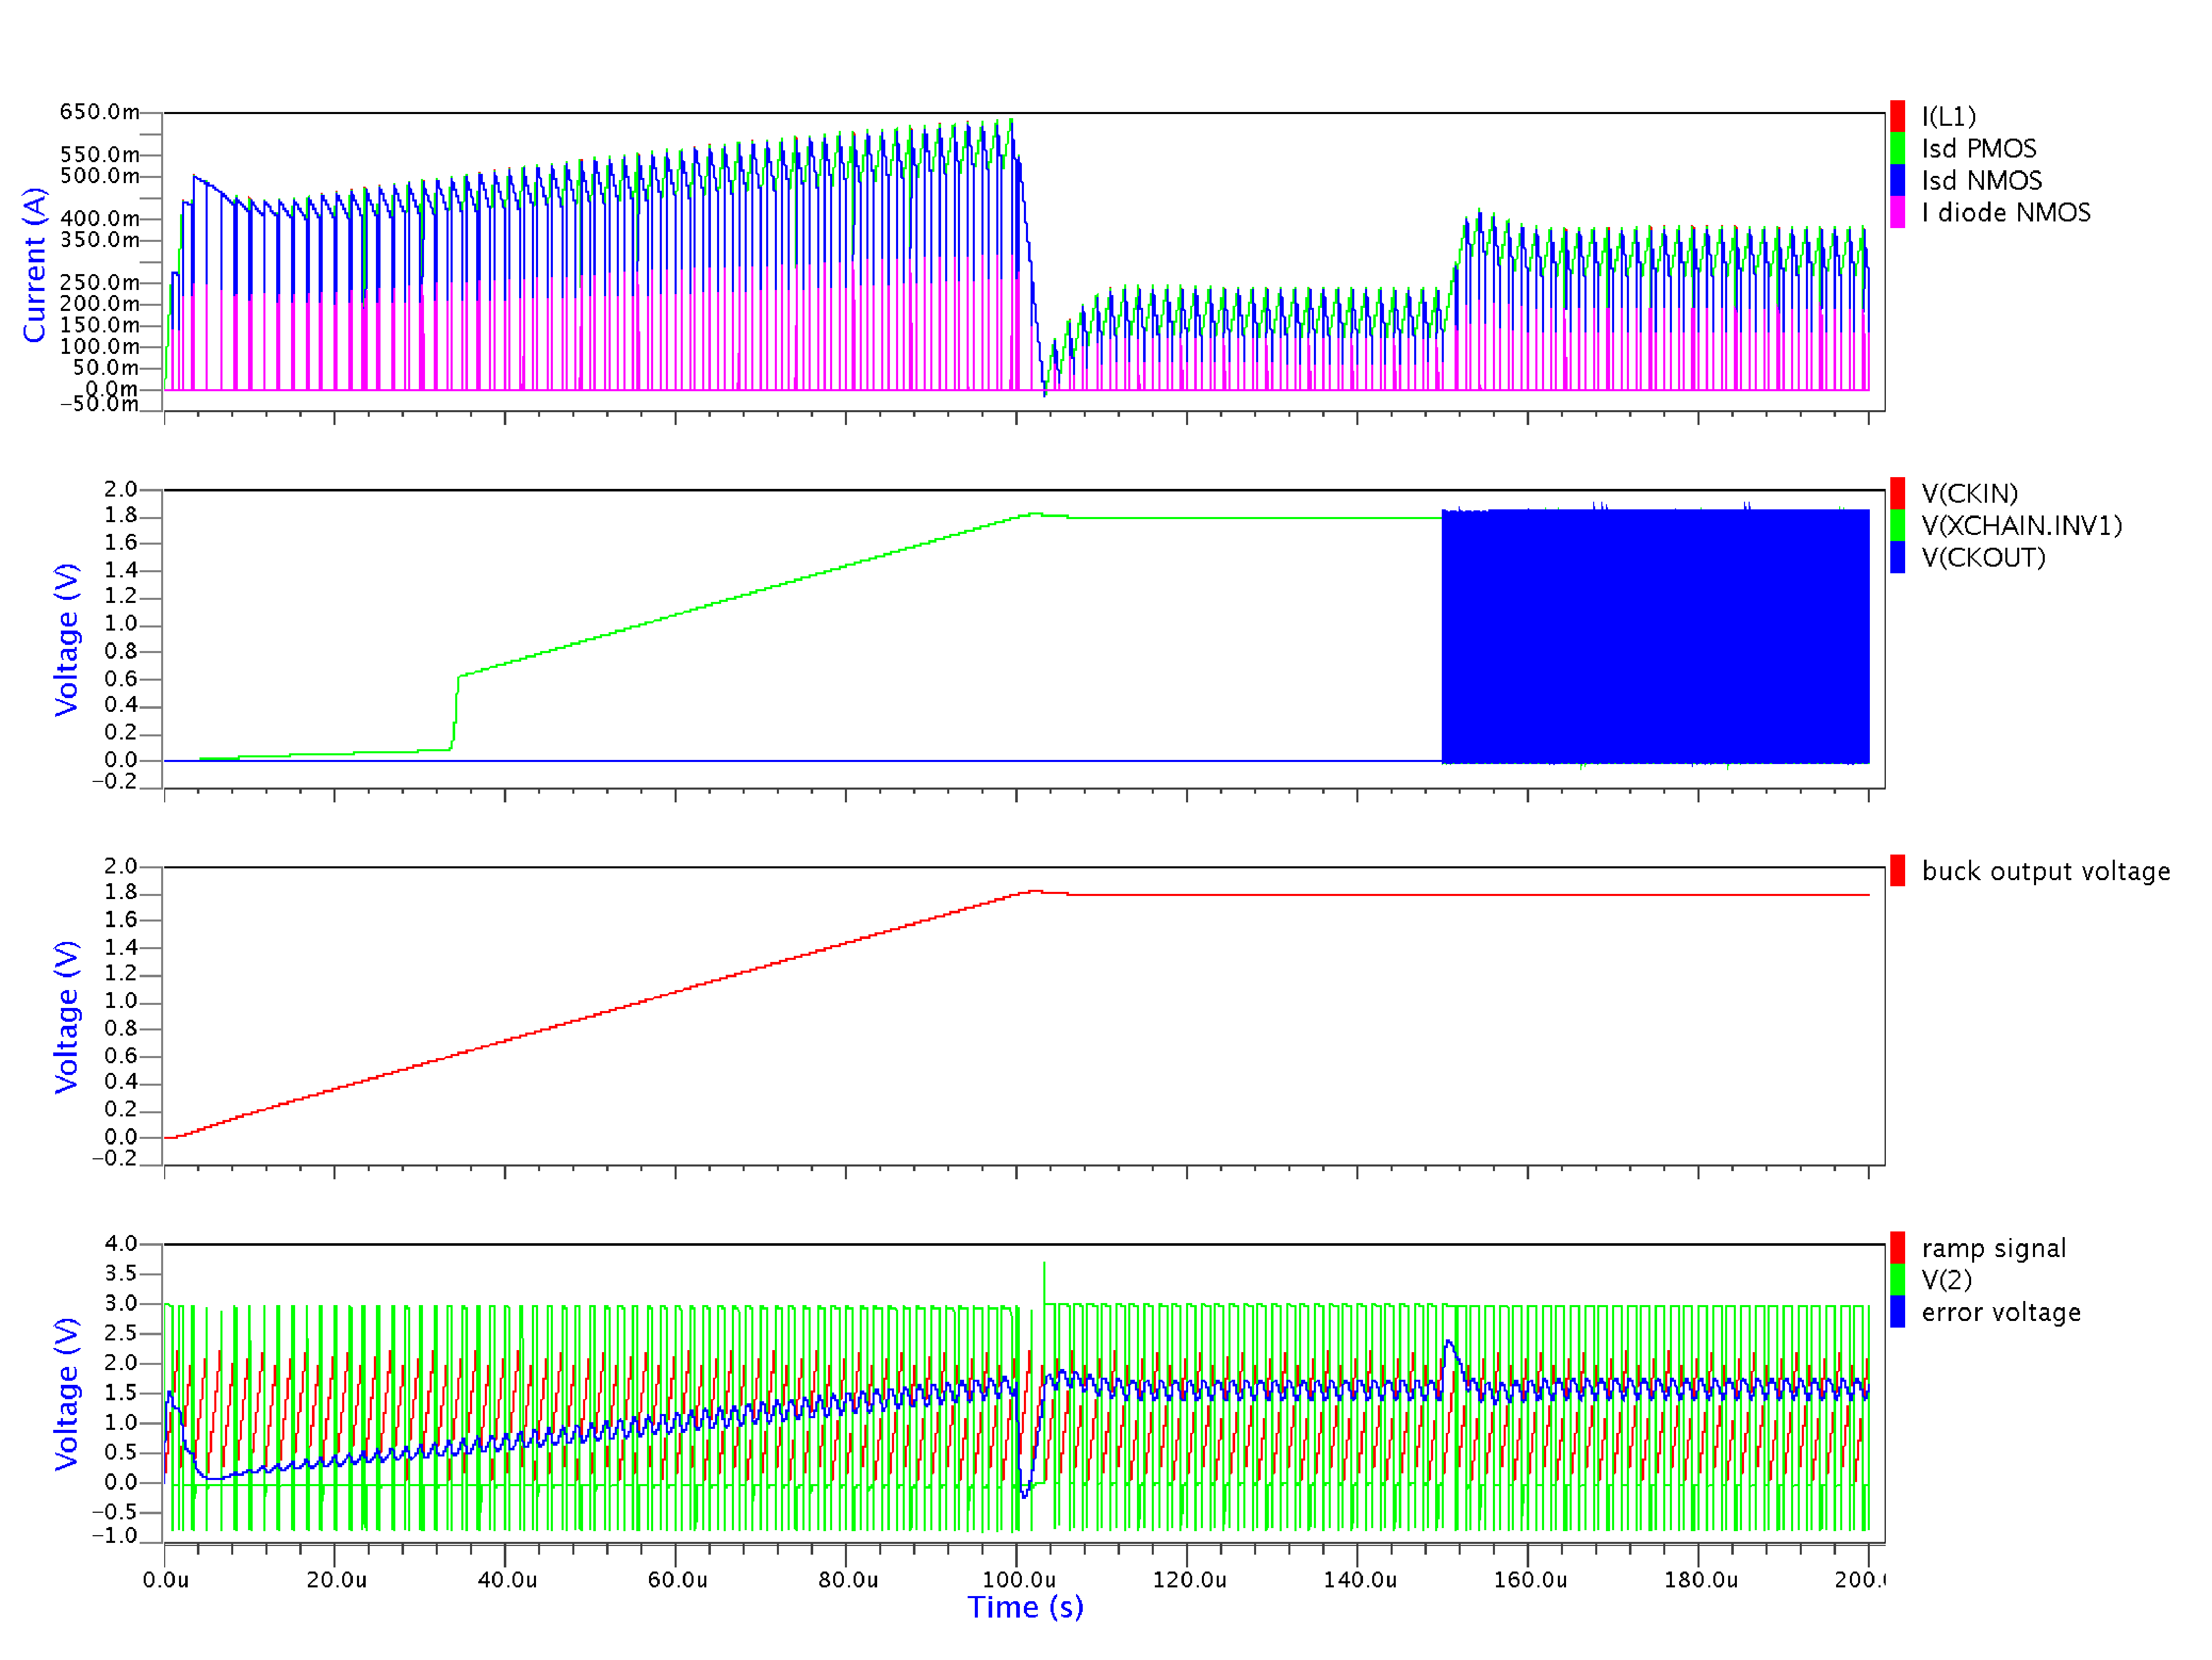
\includegraphics[scale=0.2,angle=0]{simu_ELDO_buck2inv_0p2ms_0p05ns.eps}
\end{center}
\caption[ELDO results, buck \protect\& load resistor \protect\& inverters (first~$200~\mu s$)]
{ELDO simulation results, buck converter supplying a load resistor and an inverter chain (first~$200~\mu s$)}
\label{fig-buck-inverter-simu-ELDO-0p2ms-0p05ns}
\end{figure}

\begin{figure}[hbtp]
\begin{center}
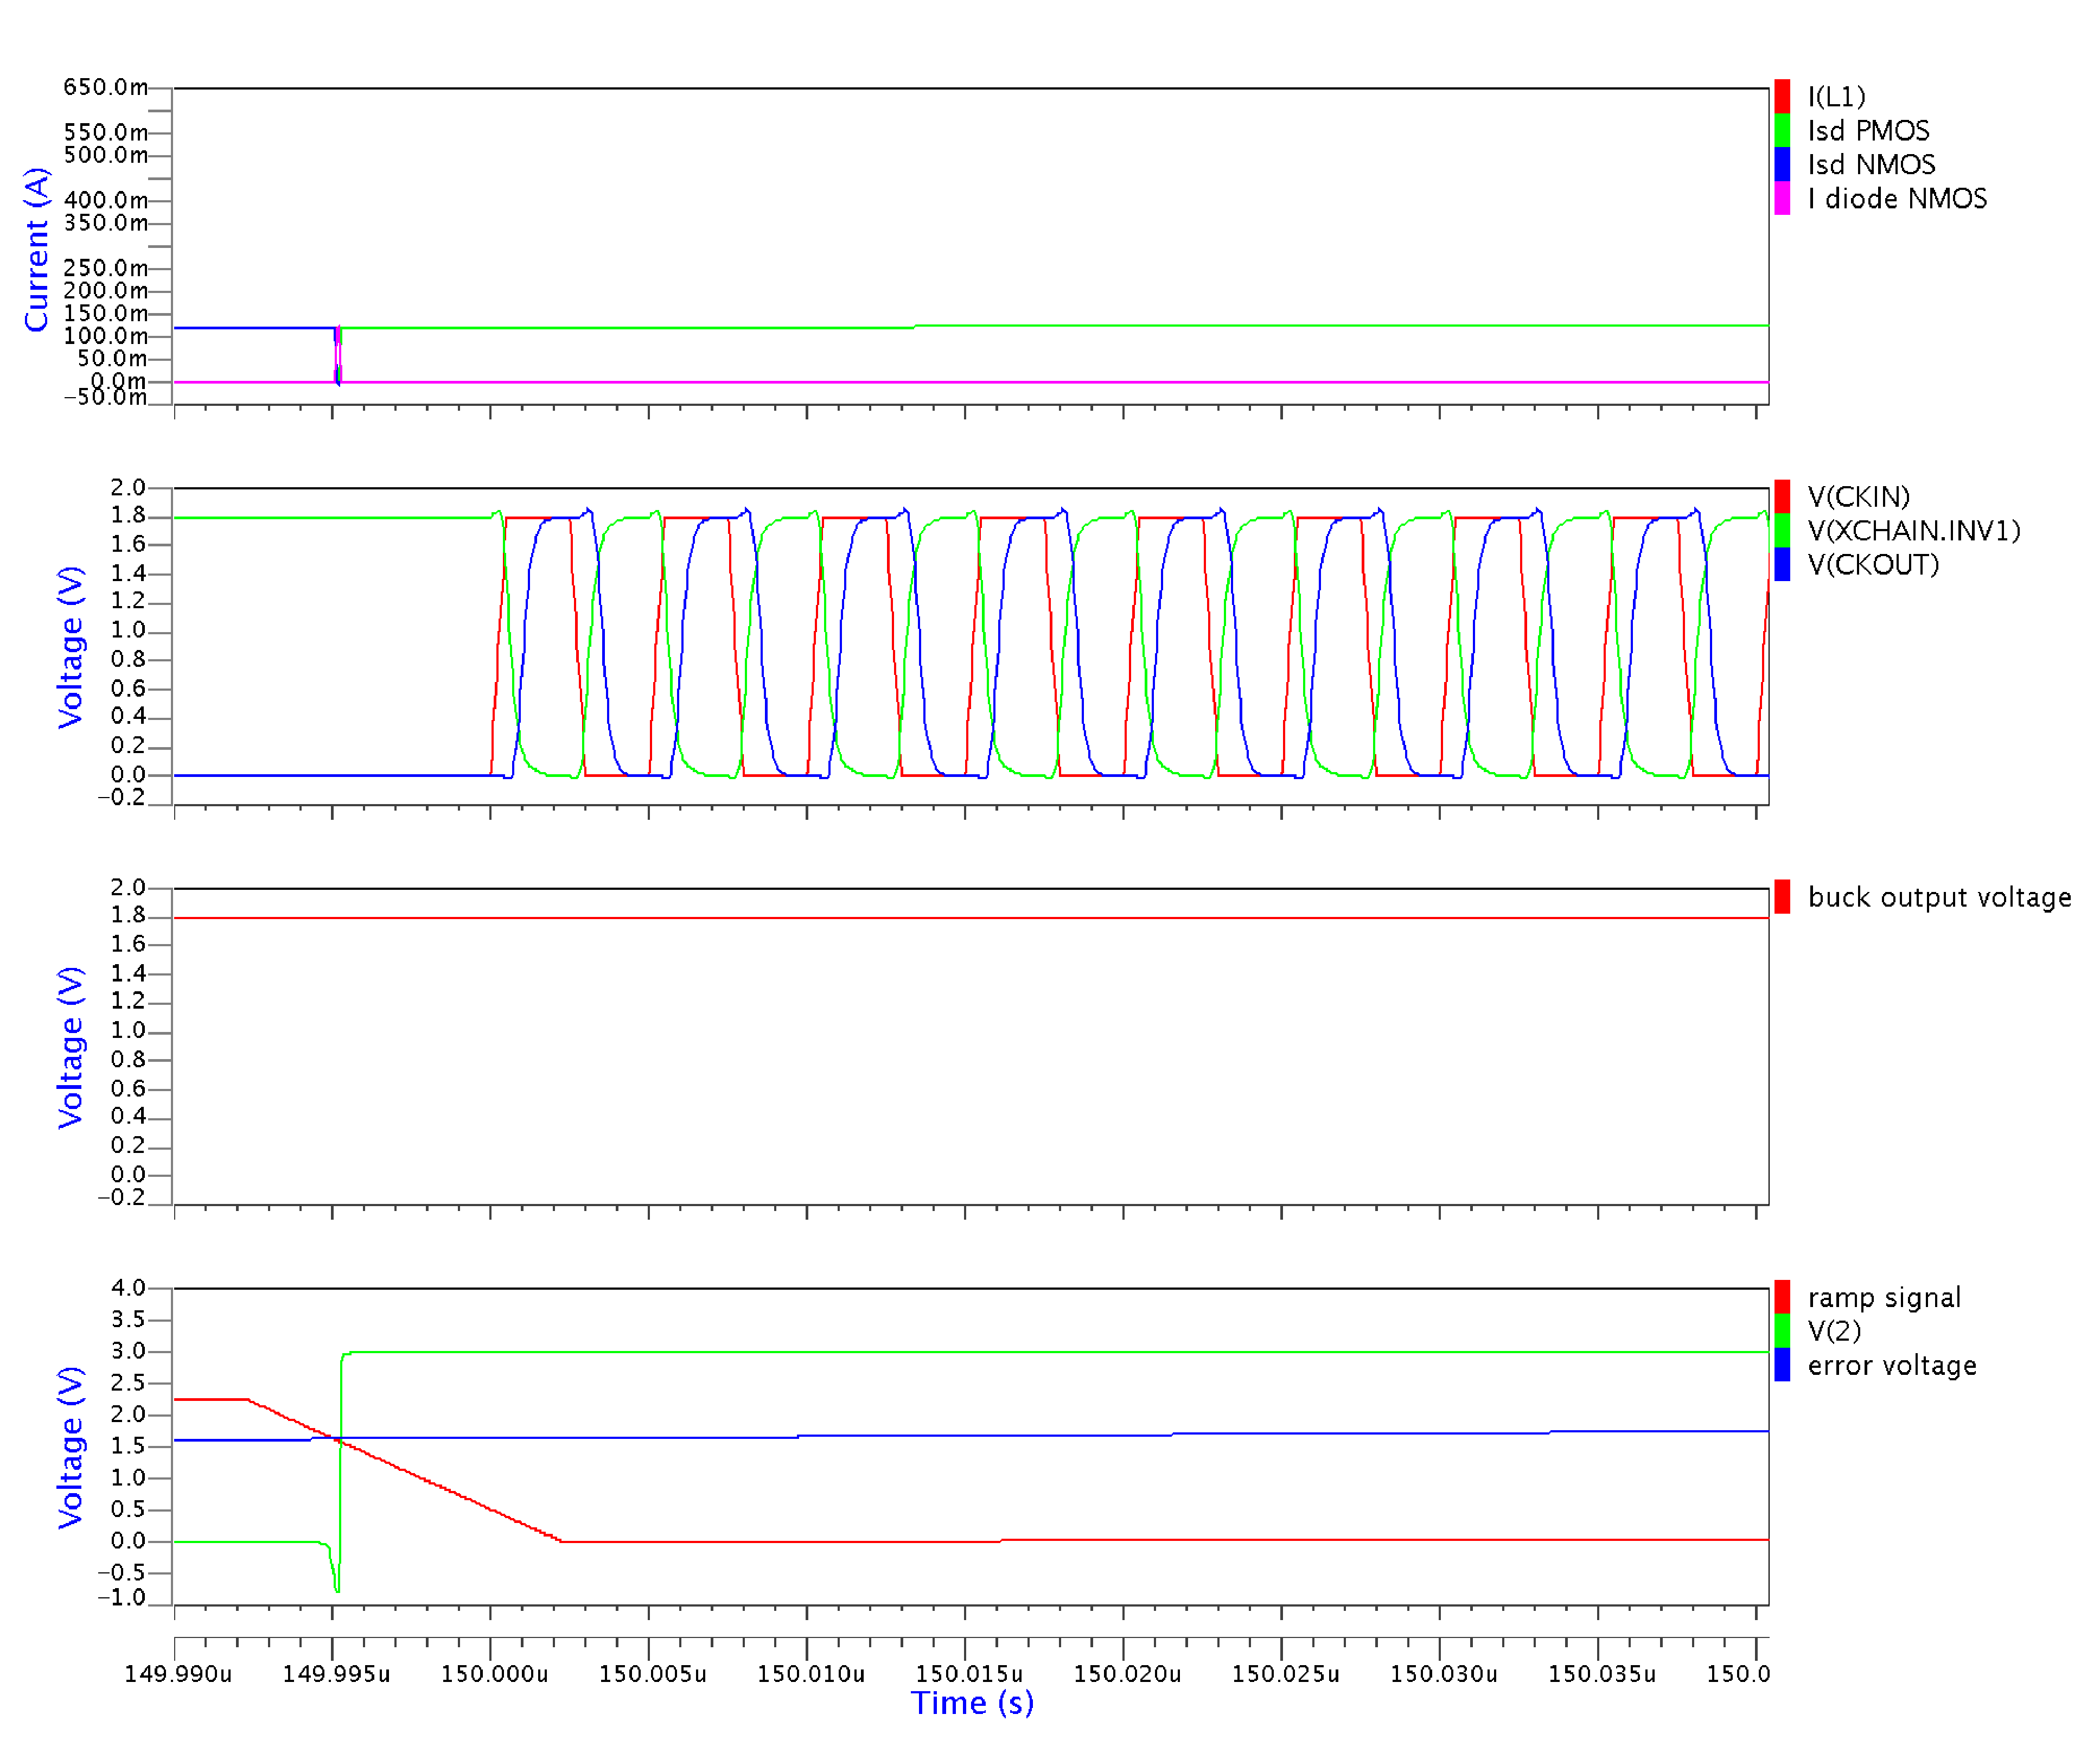
\includegraphics[scale=0.2,angle=0]{simu_ELDO_buck2inv_zoom1.eps}
\end{center}
\caption[ELDO results, buck \protect\& load resistor \protect\& inverters (zoom)]
{ELDO simulation results, buck converter supplying a load resistor and an inverter chain\protect\newline
Zoom on the start-up of the inverter chain}
\label{fig-buck-inverter-simu-ELDO-zoom1}
\end{figure}

\clearpage

\section{Simulation with PLECS}
Only 2 inverters could be used due to limitations of the evaluation version.
The inverter MOS transistors are ideal switches with a $R_{ON}$ value of~$0.54~\Omega$ to match
approximately the transconductance of the~8000~parallel MOS modelled in SICONOS. The load capacitor
is set to~$8000~\times~20~fF~=~0.16~nF$ (see description of the PLECS circuit and the Simulink model in appendix
\ref{modele-PLECS-buckinverters}).
\\
\\
\textbf{The CPU time required to achieve the simulation of~$200~\mu s$ is~$4~hours~8~min$ on a Pentium~4 clocked at 3~GHz},
i.e~135~times the SICONOS simulation time with moreover the aforementioned limitation in precision. For instance,
the ideal representation of the MOS transistors forbid to analyze voltage-depending delays in CMOS inverters, an
effect that was correctly shown with SICONOS simulation (see \ref{section-simu-siconos-buckinv}).

Results are displayed in figures \ref{fig-buck-inverter-simu-plecs-std0p2ms} and 
\ref{fig-buck-inverter-simu-plecs-stdzoom}.

\begin{figure}[hbtp]
\begin{center}
\includegraphics[scale=0.8,angle=270]{simu_plecs_buckinverters_std0p2ms.eps}
\end{center}
\caption[PLECS results, buck \protect\& load resistor \protect\& inverters (first~$200~\mu s$)]
{PLECS simulation results, buck converter supplying a load resistor and an inverter chain (first~$200~\mu s$)}
\label{fig-buck-inverter-simu-plecs-std0p2ms}
\end{figure}

\begin{figure}[hbtp]
\begin{center}
\includegraphics[scale=0.8,angle=270]{simu_plecs_buckinverters_stdzoom.eps}
\end{center}
\caption[PLECS results, buck \protect\& load resistor \protect\& inverters (zoom)]
{PLECS simulation results, buck converter supplying a load resistor and an inverter chain\protect\newline
Zoom on the start-up of the inverter chain}
\label{fig-buck-inverter-simu-plecs-stdzoom}
\end{figure}

\chapter{Conclusion}
A full buck converter supplying both a constant load and a small switching circuit was simulated
using three different classes of algorithms :

\begin{description}
\item[The SICONOS approach] allows to perform simulations in reasonable time, and thus to do quickly parametric studies
while keeping the modelling of the main characteristics of components. Furthermore, the implementation of the platform
is far from being optimized. Future major enhancements like sparse matrix techniques or Non-Linear Complementarity Problem
solvers will very likely reduce the CPU time without impairing accuracy.
\item[The SPICE approach] may lead to failures if the models are very non-linear like diodes or the variable
capacitances in the MOS level~1 model. Some simulators converge only if the circuit is regularized by
adding smoothing elements like capacitors. When convergence was reached, CPU time was at least 3~times
larger than SICONOS on small circuits. On a larger circuit with tens of nodes, SPICE results are better than
the current SICONOS version, this probably comes mainly from the use of sparse matrices.
\item[The PLECS approach] enables to simulate a low number of switches in an acceptable time provided that events
are not too frequent. When fast clocked circuitry is added, CPU time rises high, and it probably happens also
when the number of switches is increased.\footnote{The evaluation version is limited to 6 switches.}
Moreover, the models of active devices like MOS transistors are ideal thus forbidding to analyze
some effects.
\end{description}

\newpage
The CPU time and convergence results are summarized hereafter :
\\
\\
\begin{tabular}{|p{3cm}|p{3cm}|p{3cm}|p{3cm}|}
\hline
 & \textbf{SICONOS} & \textbf{SPICE (ELDO)} & \textbf{PLECS} \\
\hline
Buck converter & 52 s & 363 s  & 135 s to 410 s \\
load : resistor & {\small slightly approximate } & {\small precise } & {\small very approximate } \\
\hline
Buck converter & 110 s & 439 s & 4 hours 8 min \\
load : resistor \& inverters  & {\small slightly approximate } & {\small precise }  & {\small very approximate }\\
\hline
\end{tabular}
\newline
\newline

By ``\textit{very approximate}'', we mean that PLECS models the MOS behavior as fully ideal : it acts as an open or closed
switch controlled by a boolean signal.

By ``\textit{slightly approximate}'', we mean that SICONOS models the MOS behavior electrically with a piecewise
linear characteristic $I_{DS} = f(V_{GS},V_{DS})$.

\appendix

\chapter{PLECS/Simulink model of the buck converter with a load resistor}
\label{modele-PLECS-buckresistor}

\begin{figure}[hbtp]
\begin{center}
\includegraphics[scale=0.8,angle=270]{circuitPLECS.eps}
\end{center}
\caption{PLECS circuit part of the buck converter with a load resistor}
\end{figure}

\begin{figure}[hbtp]
\begin{center}
\includegraphics[scale=0.8,angle=270]{modeleSimulinkBuckResistor.eps}
\end{center}
\caption{Simulink model of the buck converter with a load resistor}
\end{figure}

\chapter{PLECS/Simulink model of the buck converter supplying a resistor and inverters}
\label{modele-PLECS-buckinverters}

\begin{figure}[hbtp]
\begin{center}
\includegraphics[scale=0.8,angle=270]{circuitBuckInvertersPLECS.eps}
\end{center}
\caption{PLECS circuit part of the buck converter supplying a resistor and inverters}
\end{figure}

\begin{figure}[hbtp]
\begin{center}
\includegraphics[scale=0.8,angle=270]{modeleBuckInvertersPLECS.eps}
\end{center}
\caption{Simulink model of the buck converter supplying a resistor and inverters}
\end{figure}

\bibliographystyle{alpha}
\bibliography{biblio}

\listoffigures

\end{document}
